
\setcounter{chapter}{4}
\chapter{Adição e subtração de frações }

\section{EXPLORANDO O ASSUNTO }

\setcounter{subsection}{0}
\subsection{Atividade}


Miguel e Alice estão participando de uma campanha da escola para coleta de óleo de cozinha. O objetivo é disponibilizar recipientes para que as pessoas depositem óleo. Depois esses recipientes serão destinados a empresas que usarão o óleo descartado para fazer sabão. Eles conseguiram diferentes recipientes e agora desejam saber qual tem maior capacidade.


\begin{tabular}{ccc}
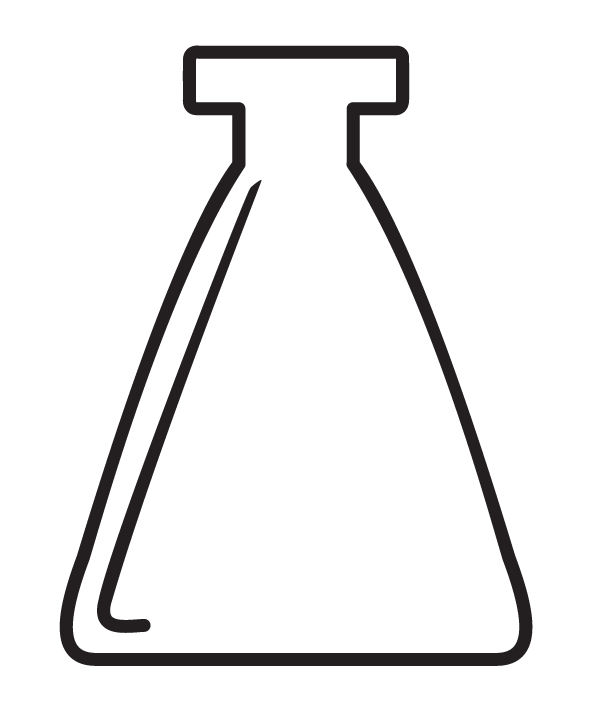
\includegraphics[width=100pt, keepaspectratio]{..//media/cap5/secoes/PNGs_licao_05/ativ1_fig01.png} &\quad \quad&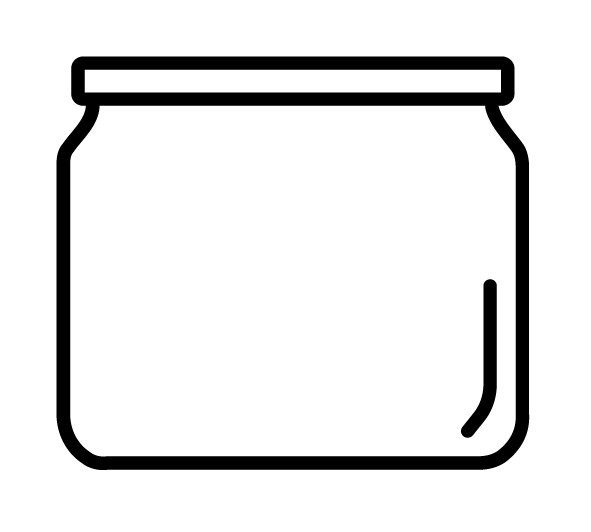
\includegraphics[width=100pt, keepaspectratio]{..//media/cap5/secoes/PNGs_licao_05/ativ1_fig02.png}\\
{\bf Recipiente 1:} trazido pela Alice & & {\bf Recipiente 2:} trazido pelo Miguel 
\end{tabular} 

Eles tiveram a seguinte ideia: encheram os dois recipientes com água para depois verificarem onde havia mais água. Para isso, usaram um copo d'água como unidade de medida. 
\begin{itemize}
 \item O recipiente trazido por Alice foi enchido com 26 copos.
 \item O recipiente trazido por Miguel foi enchido com 40 copos.
\end{itemize}
Eles então observaram que a partir de {\bf uma unidade de medida comum} (nesse caso o copo), poderiam não só dizer qual recipiente tinha maior capacidade, mas também o quanto era maior e qual seria a capacidade dos dois recipientes juntos. 
Usando a ideia de medida de Miguel e Alice, isto é, tomando o copo como unidade de medida, responda:
  \begin{enumerate}[a)]
   \item Qual recipiente tem maior capacidade?
   \item Qual é a capacidade dos dois recipientes juntos?
   \item Quanto de água se deve retirar do recipiente maior, para ter o mesmo volume de líquido que é possível colocar no recipiente menor?
  \end{enumerate}


\subsection{Atividade}

A professora Estela quer enfeitar sua sala de aula para uma festa da escola. Para isso ela comprou várias fitas, todas de mesmo tamanho, nas cores vermelho, azul e amarelo.
  
\begin{center}
\begin{tikzpicture}[x=1.0cm,y=1.0cm, scale=.5]
\draw[fill=attention] (0.,1) rectangle (12.,3.); 
\draw[fill=common] (0.,-2) rectangle (12.,0.);
\draw[fill=yellow,fill opacity=.3] (0.,-5) rectangle (12.,-3.);
\end{tikzpicture}
\end{center}


A professora cortou cada fita vermelha em 3 partes iguais, cada fita azul em 2 partes iguais e cada fita amarela em 4 partes iguais.

\begin{center}
\begin{tikzpicture}[x=1.0cm,y=1.0cm, scale=.5]
\draw[fill=attention] (0.,1) rectangle (12.,3.); 
\foreach \x in {4,8} \draw[dashed] (\x,1) -- (\x,3);
\draw[fill=common] (0.,-2) rectangle (12.,0.);
\draw[dashed] (6,-2) -- (6,0);
\draw[fill=yellow,fill opacity=.3] (0.,-5) rectangle (12.,-3.);
\foreach \x in {3,6,9} \draw[dashed] (\x,-5) -- (\x,-3);
\end{tikzpicture}
\end{center}

\begin{enumerate} [\quad a)] %s
  \item     A que fração da fita original corresponde cada pedaço recortado pela professora Estela?   
 \end{enumerate}
  
 Em seguida, a professora Estela começou a juntar pedaços recortados das fitas, formando novas fitas coloridas. Ela começou juntando (de forma intercalada) um pedaço azul e dois pedaços amarelos.     \mbox{} \newline      

\begin{center}
\begin{tikzpicture}[x=1.0cm,y=1.0cm, scale=.5]
\draw[fill=yellow,fill opacity=.3] (0.,0) rectangle (3,2);
\draw[fill=common] (3,0) rectangle (9.,2.);
\draw[fill=yellow,fill opacity=.3] (9,0) rectangle (12,2);
\end{tikzpicture}
\end{center}

Ela verificou que a nova fita formada tinha o mesmo tamanho da fita original. Isso aconteceu porque cada pedaço azul tem o mesmo tamanho de dois pedaços amarelos. Podemos representar o tamanho da nova fita formada pela professora por meio de uma {\bf soma de frações}. Cada pedaço azul corresponde a $\frac{1}{2}$ da fita original. Cada pedaço amarelo corresponde a $\frac{1}{4}$ da fita original, então 2 pedaços amarelos correspondem a $\frac{2}{4}$ da fita original. Portanto, o tamanho da nova fita é igual a: $$\dfrac{1}{2} + \dfrac{2}{4}.$$ Mas, como $\frac{2}{4}$ é igual a $\frac{1}{2}$ (cada pedaço azul tem o mesmo tamanho de dois pedaços amarelos), então: $$\dfrac{1}{2} + \dfrac{2}{4} = \dfrac{1}{2} + \dfrac{1}{2}.$$ O resultado dessa soma $\frac{1}{2} + \frac{1}{2}$ é igual 2 pedaços de $\frac{1}{2}$, isto é, $\frac{2}{2}$ (que é igual 1). Assim: $$\dfrac{1}{2} + \dfrac{2}{4} = \dfrac{1}{2} + \dfrac{1}{2} = 1.$$ Neste caso, o resultado 1 corresponde ao tamanho da fita original.
 \begin{enumerate} [\quad a)] %s
 \item[\quad b)]    A professora também agrupou pedaços de fita, juntando 1 pedaço amarelo e 1 pedaço azul, como na figura abaixo. A qual fração da fita inicial correspondem esses dois pedaços juntos?
\end{enumerate} %s

\begin{center}
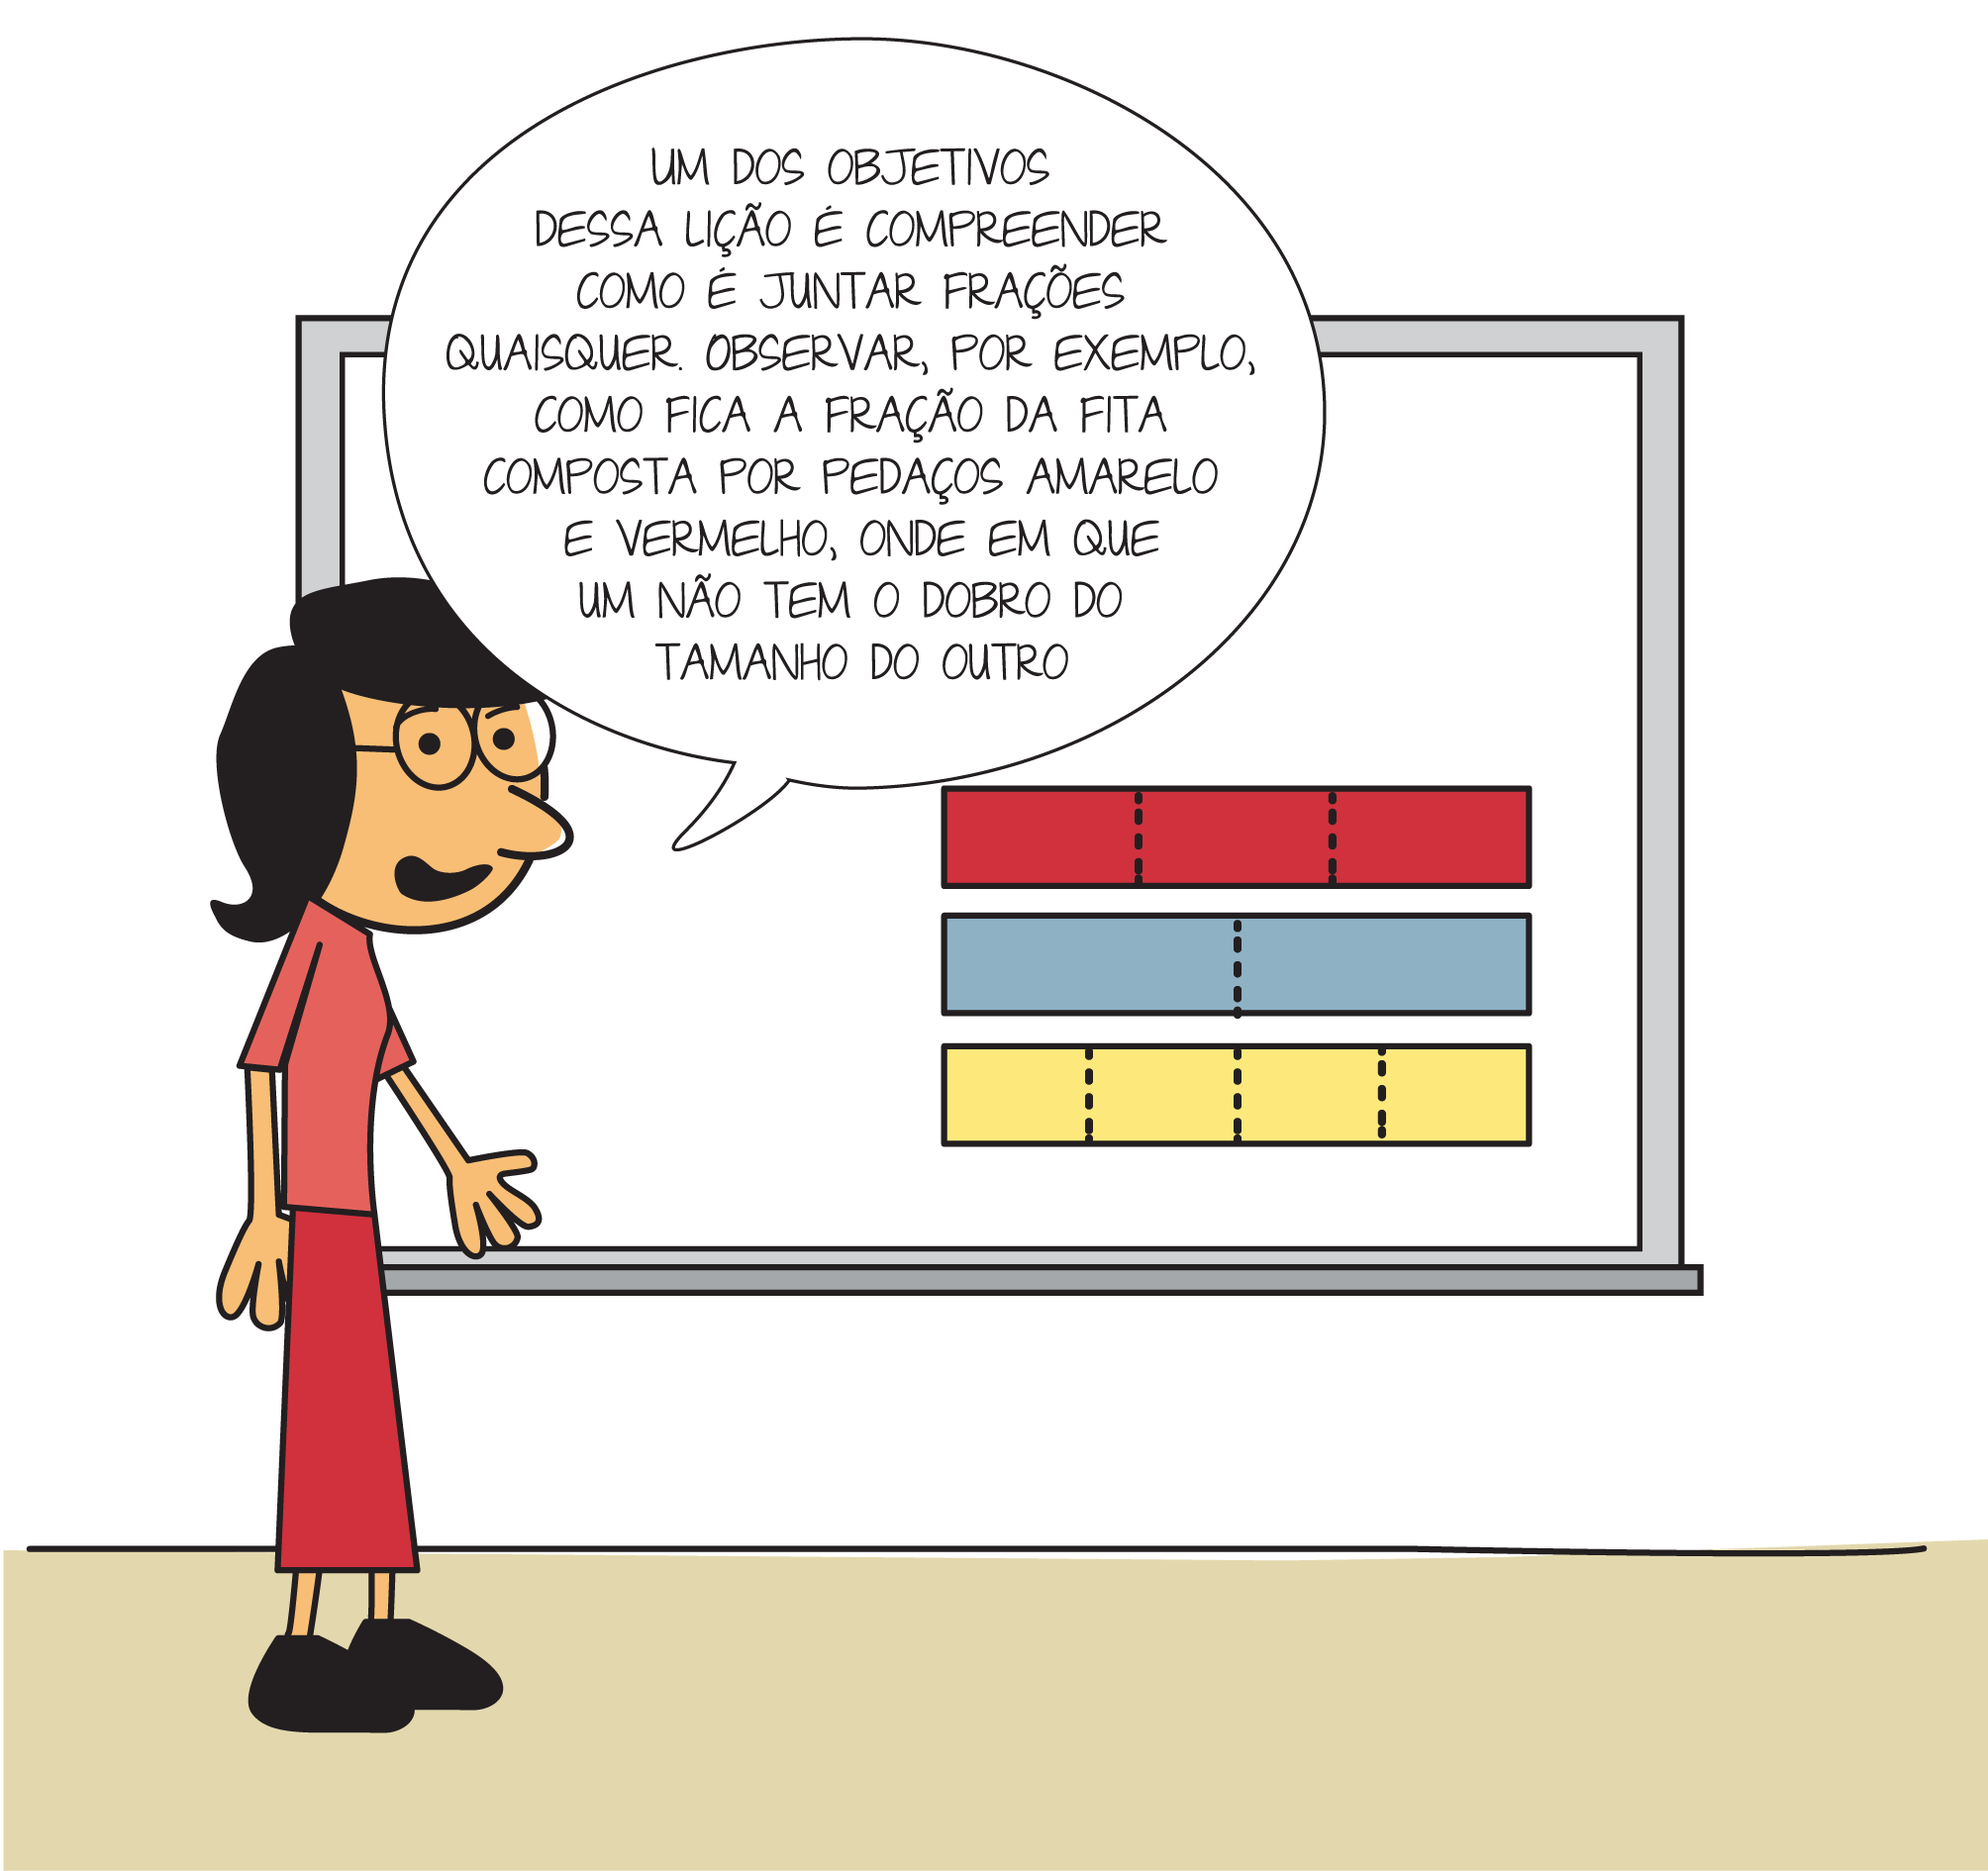
\includegraphics[width=330pt, keepaspectratio]{..//media/cap5/secoes/PNGs_licao_05/ativ2_fig01.png}
\end{center}


\subsection{Atividade}


Uma barra de chocolate é vendida com as marcações mostradas na figura abaixo.
 \begin{center}
 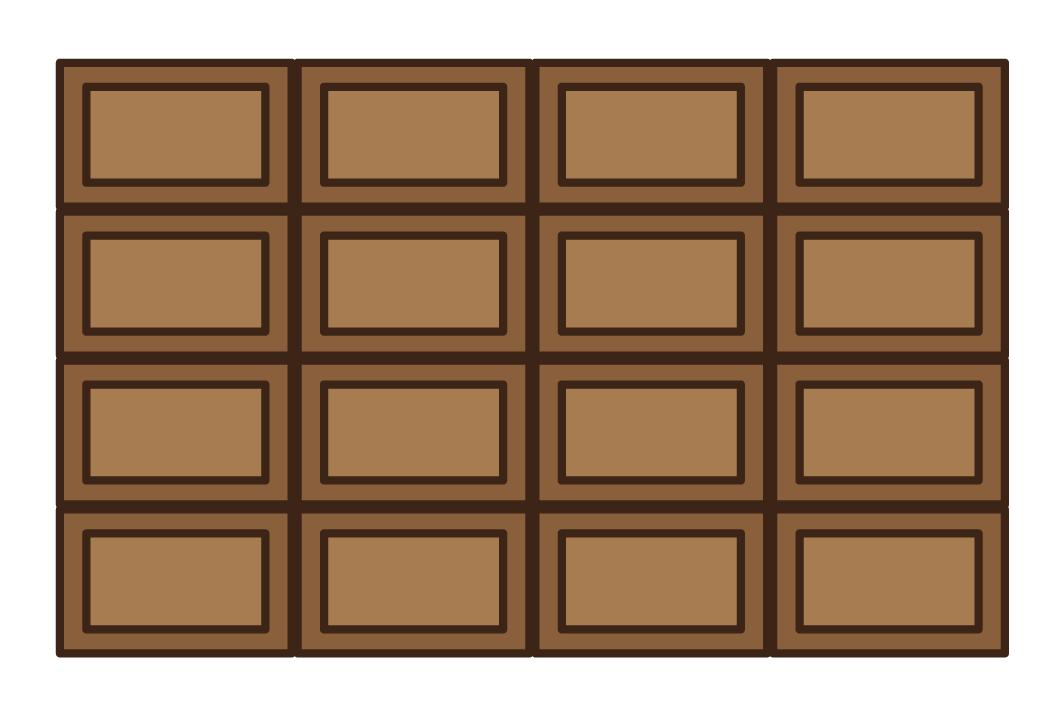
\includegraphics[width=150pt, keepaspectratio]{..//media/cap5/secoes/PNGs_licao_05/ativ3_fig01.png}
 \end{center}
 

Alice comeu a metade dessa barra de chocolate (em bege), quebrou o restante da barra em pedaços, seguindo as marcações e comeu 3 desses pedaços (em azul).

\begin{center}
\begin{tikzpicture}[x=1.0cm,y=1.0cm, scale=.7]
\fill[fill=light] (-1.,5.) -- (-1.,1.) -- (3.,1.) -- (3.,5.) -- cycle;
\fill[fill=common] (3.,5.) -- (5.,5.) -- (5.,3.) -- (3.,3.) -- cycle;
\fill[fill=common] (5.,5.) -- (7.,5.) -- (7.,4.) -- (5.,4.02) -- cycle;
\draw  (-1.,5.)-- (-1.,1.);
\draw  (-1.,1.)-- (3.,1.);
\draw  (3.,1.)-- (7.,1.);
\draw  (7.,1.)-- (7.,5.);
\draw  (7.,5.)-- (-1.,5.);
\draw  (3.,5.)-- (3.,3.);
\draw  (5.,5.)-- (5.,1.);
\draw  (-1.,3.)-- (7.,3.);
\draw  (-1.,2.)-- (7.,2.);
\draw  (1.,5.)-- (1.,1.);
\draw  (-1.,4.)-- (7.,4.);
\draw  (3.,3.)-- (3.,1.);
\end{tikzpicture}
\end{center}

Se considerarmos a barra de chocolate como a unidade, indicamos que as quantidades comidas são: $\frac{1}{2}$ por Alice e $\frac{3}{16}$ por Miguel.
Os pedaços da barra (quebrados por Miguel de acordo com as marcações na barra) correspondem a uma subdivisão dessa unidade.
Observe que ambas as frações da barra de chocolate comidas por Alice e Miguel podem ser obtidas a partir dessa subdivisão: Miguel comeu 3 pedaços e a quantidade comida por Alice corresponde a 8 pedaços.
\begin{enumerate}[a)]
\item Um pedaço corresponde a que fração da barra de chocolate?
\item Complete a parte em branco (numerador) para indicar a fração da barra de chocolate que Alice comeu. 
$$\frac{1}{2} = \frac{\text{\Large $\square$} }{16}$$ 
\item Que fração da barra de chocolate foi comida por Alice e por Miguel, juntos?
\item  Que fração da barra de chocolate não foi comida?
\end{enumerate}

\subsection{Atividade}


Amanda, Bruno e Caio pediram três pizzas do mesmo tamanho, mas com sabores diferentes. Todas as pizzas nessa pizzaria são servidas em {\bf 12 fatias} iguais. Amanda comeu $\frac{1}{6}$ de uma pizza, Bruno comeu $\frac{3}{4}$ de outra, e Caio comeu $\frac{2}{3}$ da pizza que pediu.

\begin{tabular}{m{.3\textwidth}m{.3\textwidth}m{.3\textwidth}}
 
\begin{tikzpicture}
\fill[light, opacity = .8] (0,0) -- (30:20) arc (30:90:20) --cycle;
\foreach \x in {0,60,120}{ \draw (\x:20) -- (\x:-20);}
\foreach \x in {30,90,150}{ \draw[very thick, light] (\x:20) -- (\x:-20);}
\draw[|-|] (30:25) arc (30:90:25);
\node[] at (60:30) {$\dfrac{1}{6}$};
\draw (0,0) circle (20);
\end{tikzpicture}

&
\begin{tikzpicture}
\fill[common, opacity = .8] (0,0) -- (-180:20) arc (-180:90:20) --cycle;
\foreach \x in {0,30,60,120,150}{ \draw (\x:20) -- (\x:-20);}
\foreach \x in {0,90}{ \draw[very thick, common] (\x:20) -- (\x:-20);}
\draw[|-|] (0:25) arc (0:90:25);
\node[] at (45:30) {$\dfrac{1}{4}$};
\draw (0,0) circle (20);
\end{tikzpicture}
&
\begin{tikzpicture}
\fill[special, opacity = .8] (0,0) -- (-150:20) arc (-150:90:20) --cycle;
\foreach \x in {0,30,60,90,120,150}{ \draw (\x:20) -- (\x:-20);}
\foreach \x in {-30,90,210}{ \draw[very thick, special] (0,0) -- (\x:20);}
\draw[|-|] (-30:25) arc (-30:90:25);
\node[] at (30:30) {$\dfrac{1}{3}$};
\draw (0,0) circle (20);
\end{tikzpicture}
\\
 Fração de pizza consumida por Amanda $\frac{1}{6}$  & Fração de pizza consumida por Bruno $\frac{3}{4}$  & Fração de pizza consumida por Caio $\frac{2}{3}$ 
\end{tabular}

\begin{enumerate}[a)]
\item  Que fração de uma pizza cada fatia representa?
 \item Complete os espaços (numeradores) a seguir registrando outra representação para a fração de uma pizza que cada uma das crianças comeu.\\ Amanda: $\frac{1}{6} =\frac{}{12}  \quad \quad$ Bruno: $\frac{3}{4} =\frac{}{12} \quad \quad$ Caio: $\frac{2}{3} =\frac{}{12}$ 
 \item Quem comeu mais pizza? Quem comeu menos pizza?
 \item Que quantidade de pizza Bruno comeu a mais do que Caio?
 \item Que quantidade de pizza Amanda e Bruno comeram juntas?
  \item Que fração de uma pizza Amanda comeu a menos do que Caio?
  \item Quanto a mais de pizza Bruno consumiu, em relação a Amanda?
\end{enumerate}


\section{ORGANIZANDO AS IDEIAS }

No caso de quantidades expressas por meio de frações de uma unidade dada, para comparar, determinar a soma ou determinar a diferença, é necessário uma {\bf subdivisão da unidade} com a qual seja possível expressar ambas as quantidades por meio de frações equivalentes às frações dadas e de mesmo denominador. Por exemplo:
\begin{itemize} %s
  \item     Na Atividade 3, a subdivisão da unidade considerada, barra de chocolate, permitiu expressar as quantidades de chocolate comidas por Alice e por Miguel a partir da contagem da mesma subdivisão da unidade. A partir dessa estratégia, foram determinadas a quantidade de chocolate comidas por Alice e Miguel juntos, bem como a quantidade de chocolate restante. 
  \item     Na Atividade 4, a unidade é uma pizza e a fatia de pizza é uma subdivisão dessa unidade. Neste caso, pôde-se expressar todas as frações de pizza consumidas por Amanda, Bruno e Caio a partir de contagem dessas fatias (subdivisões da unidade). Relembrando:
\end{itemize} %s

$$\dfrac{1}{6} = \dfrac{2}{12} 	\quad \quad \dfrac{3}{4} = \dfrac{9}{12} \quad \quad \dfrac{2}{3} = \dfrac{8}{12}.$$


Como os exemplos acima ilustram, a escolha adequada de uma subdivisão da unidade que permita representar as frações dadas com um mesmo denomindador foi a estratégia usada para calcular a adição e a subtração dessas frações. É exatamente essa estratégia que usaremos para calcular adição e subtração de frações em geral. 

$$\dfrac{1}{6} + \dfrac{3}{4} = \dfrac{2}{12} + \dfrac{9}{12} = \dfrac{11}{12}.$$


\section{MÃO NA MASSA }

\subsection{Atividade}

Tendo como unidade um mesmo retângulo, as representações das frações $\frac{3}{5}$ e $\frac{7}{10}$ estão ilustradas nas figuras a seguir. 

\begin{center}
\begin{tikzpicture}[scale=4]
\fill[fill=common, fill opacity=.3] (0,0) rectangle (10,5);
\fill[special] (0,0) rectangle (6,5);
\draw (0,0) rectangle (10,5);
\foreach \x in {2,4,...,8} \draw (\x,0) -- (\x, 5);

\begin{scope}[shift={(14,0)}]
\fill[fill=common, fill opacity=.3] (8,2.5) rectangle (10,5);
\fill[fill=common, fill opacity=.3] (6,0) rectangle (10,2.5);
\fill[light, opacity = .8] (0,0) rectangle (6,5);
\fill[light, opacity = .8] (6,2.5) rectangle (8,5);
\draw (0,0) rectangle (10,5);
\foreach \x in {2,4,...,8} \draw (\x,0) -- (\x, 5);
\draw (0,2.5) -- (10, 2.5);
\end{scope}
\end{tikzpicture}
\end{center}

\begin{enumerate} [\quad a)] %s
  \item     Determine uma subdivisão da unidade que permita expressar essas quantidades por frações com um mesmo denominador. Represente tal subdivisão nas figuras acima.
  \item     Escreva frações iguais a     $\frac{3}{5}$     e a     $\frac{7}{10}$     a partir dessa subdivisão.
  \item     Existe alguma outra subdivisão, diferente da que você usou para responder os itens a) e b), com a qual também seja possível responder ao item b)? Se sim, qual? 
  \item     Juntas, as regiões destacadas em vermelho e em bege determinam um região maior, menor ou igual a um retângulo? Explique.
\end{enumerate} %s

\subsection{Atividade}

Aqui retomamos a Atividade 2, na qual a professora Estela comprou fitas de mesmo tamanho e as cortou em partes iguais: a vermelha em três pedaços; a azul em dois pedaços e a amarela em quatro pedaços. 


\begin{center}
\begin{tikzpicture}[x=1.0cm,y=1.0cm, scale=.5]
\draw[fill=attention] (0.,1) rectangle (12.,3.); 
\foreach \x in {4,8} \draw[dashed] (\x,1) -- (\x,3);
\draw[fill=common] (0.,-2) rectangle (12.,0.);
\draw[dashed] (6,-2) -- (6,0);
\draw[fill=yellow,fill opacity=.3] (0.,-5) rectangle (12.,-3.);
\foreach \x in {3,6,9} \draw[dashed] (\x,-5) -- (\x,-3);
\end{tikzpicture}
\end{center}


\begin{enumerate}[a)]
  \item  Agora, a professora Estela juntou um pedaço da fita vermelha com um pedaço da fita azul. Essa nova fita formada tem tamanho maior ou menor ou igual ao tamanho original de uma fita? A que fração de uma fita original corresponde a nova fita vermelha e azul? Qual é a diferença entre os tamanhos de uma fita original e da fita vermelha e azul?
  \item  A professora formou então mais uma fita colorida, agora juntando (de forma intercalada) dois pedaços vermelhos e três pedaços amarelos. Essa nova fita vermelha e amarela é maior ou menor do que uma fita original? A que fração de uma fita original corresponde a nova fita vermelha e azul? Qual é a diferença entre os tamanhos da fita original e da fita vermelha e amarela?
\end{enumerate}


\subsection{Atividade}


Em cada um dos itens a seguir, escreva frações iguais às frações dadas que tenham mesmo denominador. Para cada par de frações, destaque a subdivisão escolhida da unidade para determinar o denominador comum e represente essa subdivisão por meio de um desenho.

\begin{center}
  \begin{tabular}{m{0.25\textwidth}m{0.25\textwidth}m{0.25\textwidth}}
    
     a) $\frac{1}{3}$ e $\frac{2}{9}$  &   b) $\frac{3}{10}$ e $\frac{4}{5}$  &   c) 1 e $\frac{3}{7}$  \\
     \\
     d) $\frac{3}{5}$ e $\frac{8}{3}$  &   e) $\frac{7}{8}$ e $\frac{13}{12}$  &  f) $\frac{7}{4}$ e 5     
  \end{tabular}
\end{center}

\subsection{Atividade}

Em cada um dos itens a seguir, faça a conta e uma ilustração que explique a maneira como você realizou o cálculo solicitado.

\begin{center}
  \begin{tabular}{m{0.25\textwidth}m{0.25\textwidth}m{0.25\textwidth}}    
     a) $\frac{1}{3} - \frac{2}{9}$  &   b) $\frac{3}{10} + \frac{4}{5}$  &   c) $1 - \frac{3}{7}$     
  \end{tabular}
\end{center}

\subsection{Atividade}
Miguel deseja calcular a soma $2 + \frac{1}{3}$. Para isso, marcou na reta numérica um ponto determinado pela justaposição do segmento correspondente a $2$ unidades com um segmento igual a $\frac{1}{3}$ da unidade, como na figura abaixo. 

Miguel relacionou essa estratégia com o seguinte cálculo: 
$$ 2 + \frac{1}{3} =  \frac{6}{3} + \frac{1}{3} = \frac{7}{3}$$

% 
% \begin{center}
%  \begin{tikzpicture}[x=17mm,y=17mm]
%   \draw[->] (0,-.25) -- (0,3.25);
%   \foreach \x in {0,...,3}{
%   \draw (-3pt,\x)--(3pt,\x);
%   \node at (-7pt,\x) {\x};}
%  \foreach \x in {2+1/3,2+2/3}\draw (-2pt,\x)--(2pt,\x); 
%  \draw[|-|] (9pt,2) -- (9pt,2+1/3);
%  \node at (20pt,2+1/6) {$\dfrac{1}{3}$};
%  \draw[->] (-35pt,2+1/3) -- (-9pt,2+1/3);
%  \node at (-1.1,2+1/3) {$2 + \dfrac{1}{3}$};
%  \fill[common] (0,2+1/3) circle (3pt);
%  \end{tikzpicture}
% \end{center}


\begin{center}
 \begin{tikzpicture}[x=17mm,y=17mm]
  \draw[->] (0,-.25) -- (0,3.25);
  \foreach \x in {0,...,3}{
  \draw (-3pt,\x)--(3pt,\x);
  \node at (-7pt,\x) {\x};}
 \foreach \x in {2+1/3,2+2/3}\draw (-2pt,\x)--(2pt,\x); 
 \draw[|-|] (9pt,2) -- (9pt,2+1/3);
 \node at (20pt,2+1/6) {$\dfrac{1}{3}$};
 \draw[->] (-35pt,2+1/3) -- (-9pt,2+1/3);
 \node at (-1.1,2+1/3) {$2 + \dfrac{1}{3}$};
 \fill[common] (0,2+1/3) circle (3pt);
 \draw[dotted] (9 pt, 2+1/3) -- (1.9, 2+1/3);

 \begin{scope}[shift={(2,0)}]
 %reta numerica vertical
 \draw[->] (0,-.25) -- (0,3.25);
  \foreach \x in {0,...,3}{
  \draw (-3pt,\x)--(3pt,\x);
  \node at (-7pt,\x) {\x};}
\foreach \x in {0,.3333,...,2.6666}\draw (-2pt,\x)--(2pt,\x); 
  \fill[common] (0,2+1/3) circle (3pt);

% segmentos de 1/3 ao lado da reta

\foreach \x in {1,...,6}{ 
\draw[|-|] (9pt,\x/3+.01) -- (9pt,\x/3+1/3-.01);
\node at (20pt,\x/3+1/6) {{\small $\frac{1}{3}$}};}
\draw[|-|] (9pt,0) -- (9pt,1/3-.01);
\node at (20pt,1/6) {{\small $\frac{1}{3}$}};

%flecha e texto.
\draw[<-]  (30 pt, 2+1/6) -- (56pt, 2+1/6);
\node at (90pt, 2+1/6) {1 fração de $\dfrac{1}{3}$};
\node at (90pt, 1.6) {$+$};
\node at (90pt, 1) {6 frações de $\dfrac{1}{3}$};
%linhas tracejadas e chave
\foreach \x in {0,2} \draw[dotted] (25pt,\x) -- (45pt,\x);
\draw [thick, decoration={brace,mirror,raise=5}, decorate] (45pt,0) -- (45pt,2); 
 \end{scope}
 \end{tikzpicture}
\end{center}


\begin{enumerate}[a)]
 \item Em cada item a seguir, a partir da imagem repita o procedimento feito por Miguel e realize os cálculos.
 
\begin{center} 
\begin{tabular}{m{.3\textwidth}m{.3\textwidth}m{.3\textwidth}}
 (A) & (B) & (C)\\
  
 \begin{tikzpicture}[x=17mm,y=17mm]
  \draw[->] (0,-.5) -- (0,4.5);
  \foreach \x in {0,...,4}{
  \draw (-3pt,\x)--(3pt,\x);
  \node at (-7pt,\x) {\x};}
 \foreach \x in {3.25,3.5,3.75}\draw (-2pt,\x)--(2pt,\x); 
 \fill[common] (0,3.25) circle (3pt);
 
 % setinha e texto
 \draw[->] (-35pt,3.25) -- (-9pt,3.25);
 \node at (-1.1,3.25) {$3 + \dfrac{1}{4}$};
 
 \end{tikzpicture}
& 

 \begin{tikzpicture}[x=17mm,y=17mm]
  \draw[->] (0,-.5) -- (0,5.5);
  \foreach \x in {0,...,5}{
  \draw (-3pt,\x)--(3pt,\x);
  \node at (-7pt,\x) {\x};}
 \draw (-2pt,4.5)--(2pt,4.5); 
 \fill[common] (0,4.5) circle (3pt);
 
 % setinha e texto
 \draw[->] (-35pt,4.5) -- (-9pt,4.5);
 \node at (-1.1,4.5) {$4 + \dfrac{1}{2}$};
  \end{tikzpicture}
 &
 \begin{tikzpicture}[x=17mm,y=17mm]
  \draw[->] (0,-.5) -- (0,3.5);
  \foreach \x in {0,...,3}{
  \draw (-3pt,\x)--(3pt,\x);
  \node at (-7pt,\x) {\x};}
 \draw (-2pt,2.6)--(2pt,2.6); 
 \foreach \x in {2.2,2.4,...,2.8}\draw (-2pt,\x)--(2pt,\x); 
 \fill[common] (0,2.6) circle (3pt);
 
 % setinha e texto
 \draw[->] (-35pt,2.6) -- (-9pt,2.6);
 \node at (-1.1,2.6) {$2 + \dfrac{3}{5}$};
 
 \end{tikzpicture}
\end{tabular}
\end{center}
 
 \item Que valor é obtido se juntarmos 7 inteiros com dois terços?
\end{enumerate}

\subsection{Atividade}


Quanto se deve acrescentar a $\frac{3}{8}$ para que se obtenha $\frac{27}{8}$?


\subsection{Atividade}

Qual é o maior número, $\frac{19}{7}$ ou $2$? Quanto se deve acrescentar ao menor número para chegar ao maior?

\subsection{Atividade}

Observando a reta, Miguel conseguiu determinar o tamanho do segmento azul entre os dois pontos $A = 3$ e $B = 7$ marcados da seguinte forma:

\begin{center}
\definecolor{DarkGreen}{rgb}{0.0, 0.5, 0.0}
\begin{tikzpicture}[x=17mm,y=17mm]
\draw[->] (-0.5,0) -- (7.5,0) ; %reta anterior
\foreach \x in {0,...,7}{ \draw (\x,3pt) -- (\x,-3pt) node[below] {\x}; }
\draw[common, line width=0.4mm] (3,0) -- (7,0);
\foreach \x in {3,7} \fill[common] (\x,0) circle (3 pt); 
\node[above] at (3,3pt) {$A$};  
\node[above] at (7,3pt) {$B$};
\node[color=attention] at (5,-30pt) {{\Large 7}};
\node[] at (5.2,-30pt) {{\Large $-$}};
\node[color=DarkGreen] at (5.4,-30pt) {{\Large 3}};
\node[] at (5.6,-30pt) {{\Large $=$}};
\node[common] at (5.8,-30pt) {{\Large 4}};
\draw[|-|, shift={(0,-30pt)},  color=DarkGreen, line width=0.4mm] (0,0)--(3,0);
\draw[|-|, shift={(0,-45pt)}, color=attention, line width=0.4mm] (0,0)--(7,0);
\end{tikzpicture}
\end{center}

Miguel calculou o tamanho do segmento azul fazendo a diferença entre o tamanho do segmento vermelho e o tamanho do segmento verde. Assim, concluiu que o tamanho do segmento AB é igual a 4.
Usando um raciocínio parecido, e considerando $C = \frac{5}{4}$ e $D=\frac{11}{6}$, ajude Miguel a realizar as tarefas a seguir.

\begin{center}
\begin{tikzpicture}[x=50mm,y=50mm]
\draw[->] (-0.25,0) -- (2.25,0) ; %reta anterior
\foreach \x in {0,1,2}{ \draw (\x,3pt) -- (\x,-3pt) node[below] {\x}; }
\draw[common, line width=0.4mm] (5/4,0) -- (11/6,0);
\foreach \x in {5/4,11/6} \fill[common] (\x,0) circle (3 pt); 
\node[above] at (5/4,3pt) {$C$};  
\node[above] at (11/6,3pt) {$D$};
\node[below] at (5/4,-3pt) {$\frac{5}{4}$};  
\node[below] at (11/6,-3pt) {$\frac{11}{6}$};
\end{tikzpicture}
\end{center}


\begin{enumerate} [\quad a)] %s
  \item     Escreva C e D a partir de uma mesma subdivisão da unidade (isto é, com o mesmo denominador).
  \item     Determine seis frações que correspondam a pontos na reta numérica entre $C$ e $D$. \newline      
  Discuta com seus colegas se é possível determinar mais que seis valores e, se for possível, qual seria a estratégia para fazer isso.
  \item     Calcule o tamanho do segmento     $CD$.
  \item     Determine uma fração que, somada a     $\frac{5}{4}$     dê um resultado menor que     $\frac{11}{6}$. Justifique a sua resposta usando a reta.     $$ \dfrac{5}{4} +\dfrac{\text{\Large $\square$}}{\text{\Large $\square$}} = \dfrac{11}{6}.$$     
  \item     Encontre outras três possíveis respostas para o item anterior. 
  \item     Determine duas frações possíveis, que quando somadas a     $\frac{5}{4}$     tenham como resultado     $\frac{11}{6}$. Justifique a sua resposta usando a reta.     $$ \dfrac{5}{4} +\dfrac{\text{\Large $\square$}}{\text{\Large $\square$}} + \dfrac{\text{\Large $\square$}}{\text{\Large $\square$}} = \dfrac{11}{6}.$$     
\end{enumerate} %s

\subsection{Atividade}

A família de Miguel reservou um determinado espaço retangular para fazer um canteiro em seu quintal. A família quer que o cateiro tenha rosas e verduras frescas. O pai de Miguel disse que precisa de $\frac{2}{3}$ do espaço inicialmente reservado, para cultivar rosas. A mãe disse que necessita de $\frac{1}{2}$ desse espaço, para plantar as verduras. Quando Miguel ouviu o diálogo dos pais, pensou nas seguintes questões:
\begin{enumerate} [\quad a)] %s
  \item     Quem precisa de mais espaço, seu pai ou sua mãe? 
  \item     O espaço reservado inicialmente para o canteiro é suficiente para comportar os espaços de que o pai e a mãe de Miguel precisam? 
  \item     Caso o espaço seja suficiente, que fração do mesmo ficaria sem uso? 
  \item     Caso o espaço não seja suficiente, que fração do canteiro reservado inicialmente deverá ser acrescentada para que a família consiga fazer as plantações que deseja? 
\end{enumerate} %s


Faça um desenho que ajude a explicar as suas respostas para as questões de Miguel. Não deixe de indicar a subdivisão da unidade que você empregou.

\subsection{Atividade}

Há três recipientes cilíndricos, de mesmo tamanho, contendo água. No primeiro recipiente, a água ocupa dois terços de sua capacidade. No segundo, a água ocupa metade de sua capacidade. No terceiro, a água ocupa cinco oitavos de sua capacidade.  
\begin{center}  
  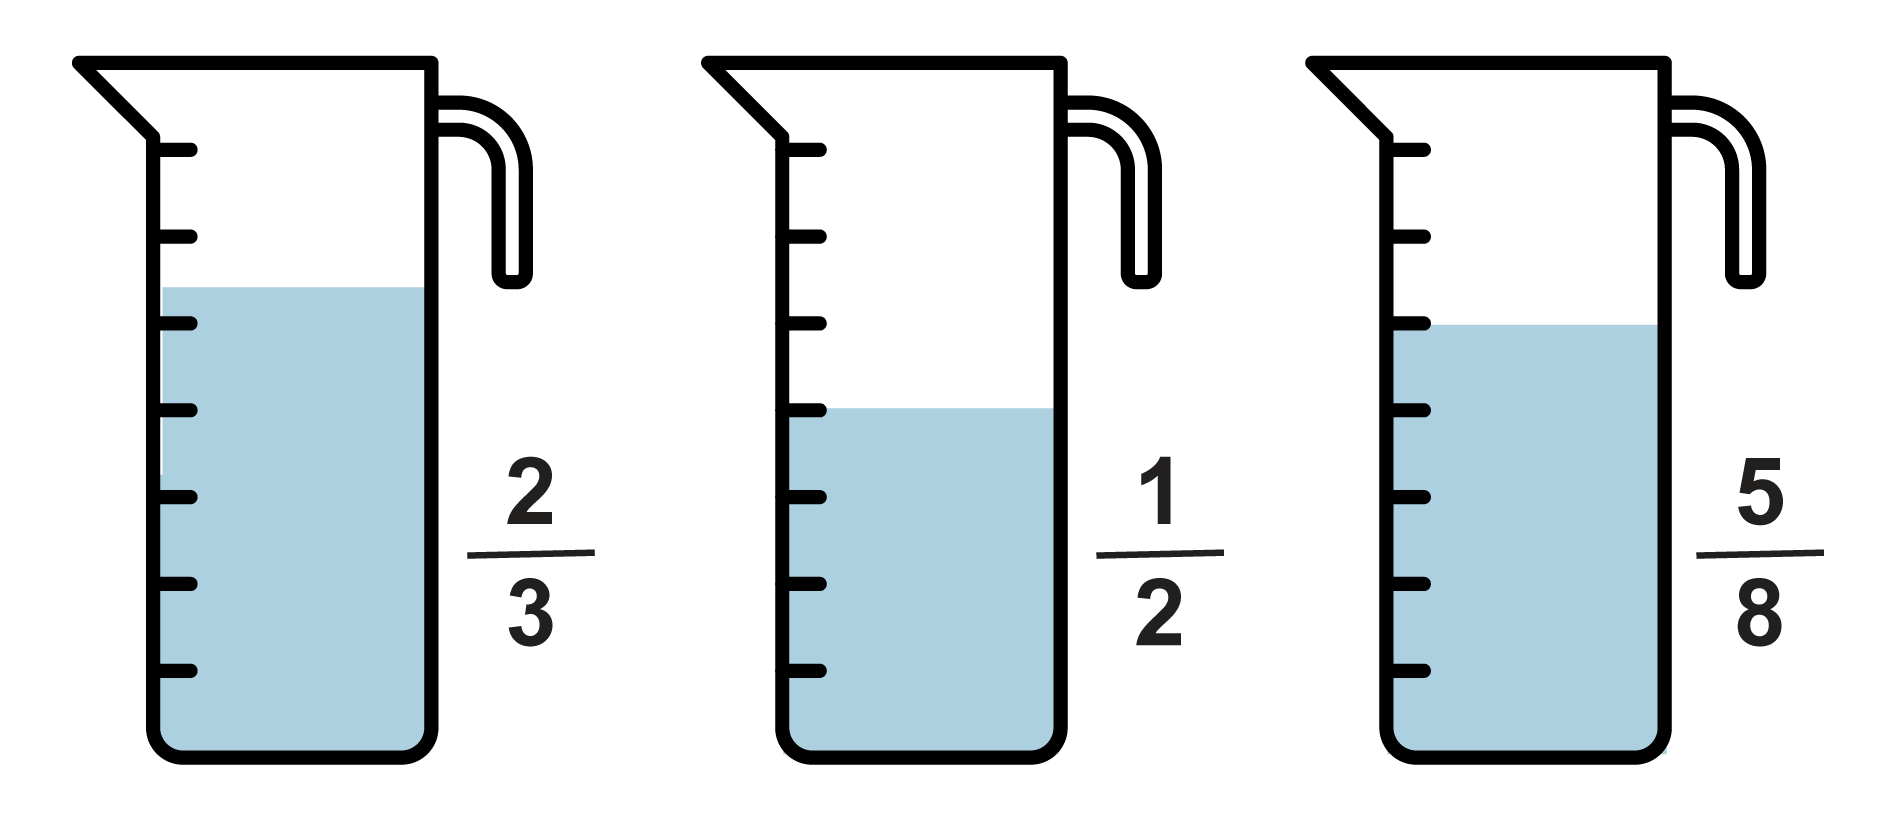
\includegraphics[width=330pt, keepaspectratio]{..//media/cap5/secoes/PNGs_licao_05/ativ14_fig01.png}
\end{center}

É possível redistribuir a água de todos os recipientes em somente dois deles?

\section{QUEBRANDO A CUCA }

\subsection{Atividade}

Diga se as afirmações a seguir são verdadeiras ou falsas. Para as verdadeiras, explique com as suas palavras por que acha que são verdadeiras. Para as falsas, dê um exemplo que justifique a sua avaliação.
\begin{enumerate} [\quad a)] %s
  \item     A soma de um número inteiro com uma fração não inteira pode sempre ser expressa por um número inteiro.
  \item     A diferença entre um número inteiro e uma fração não inteira pode sempre ser expressa por um número inteiro.
  \item     A soma de uma fração não inteira com uma fração não inteira é, necessariamente, uma fração não inteira.
  \item     A diferença entre uma fração não inteira e uma fração não inteira é, necessariamente, uma fração não inteira.
\end{enumerate} %s

